% dvisvgm --pdf name
% latexmk -C
\documentclass[preview]{standalone}
\usepackage{tikz}
\usepackage{amsmath}
\usepackage{color}
\usepackage{tabularray}
\definecolor{Sushi}{rgb}{0.545,0.756,0.294}
\definecolor{Frost}{rgb}{0.933,0.968,0.89}
\usetikzlibrary{shapes.geometric, arrows}
\tikzstyle{block} = [rectangle, rounded corners,
minimum width=3.5cm,
minimum height=2cm,
text centered, 
draw=gray]

\tikzstyle{io} = [trapezium, 
trapezium stretches=true,
trapezium left angle=70, 
trapezium right angle=110, 
minimum width=3.5cm, 
minimum height=2cm, text centered, 
draw=gray]

\tikzstyle{process} = [rectangle, 
minimum width=3.5cm,
minimum height=2cm,
text centered, 
text width=3cm, 
draw=gray]

\tikzstyle{decision} = [diamond, 
minimum width=3cm, 
minimum height=1cm, 
text centered, 
draw=gray]
\tikzstyle{arrow} = [thick,->,>=stealth]

\tikzstyle{circle} = [circle, 
minimum size=1cm, 
text centered, 
draw=gray]

\begin{document}
    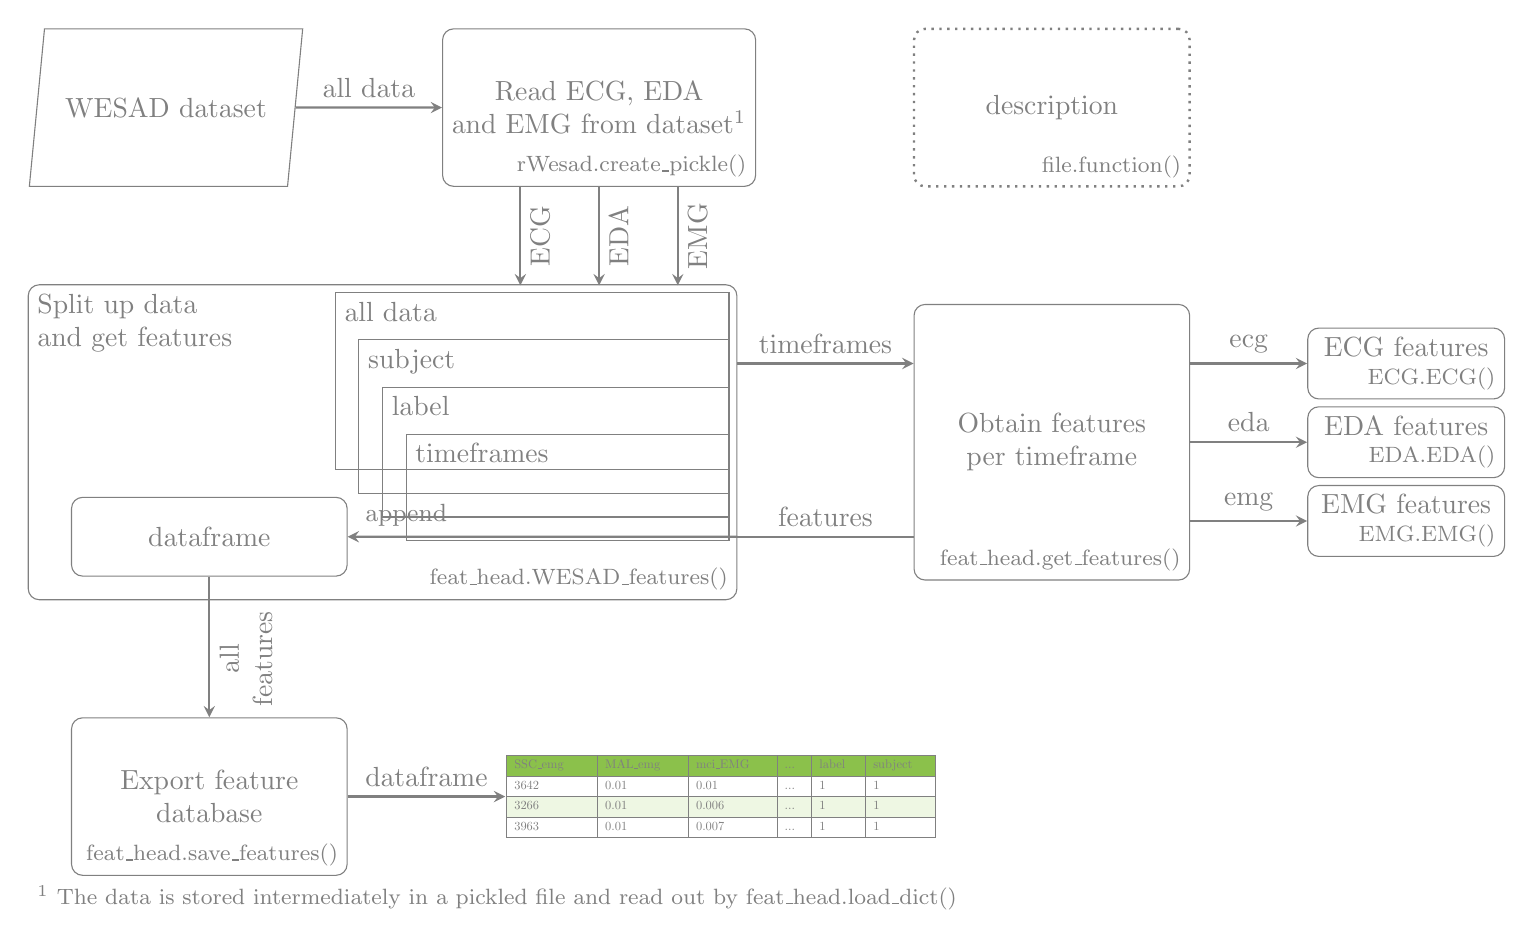
\begin{tikzpicture}[transform shape, every node/.append style={}, color=gray, node distance = 3.5cm]
        % All blocks
        \node (WESAD) [io] {WESAD dataset};

        \node (read_WESAD) [block, right of=WESAD, xshift = 2 cm, align =center] {Read ECG, EDA \\ and EMG from dataset$^{1}$};
        \node at (read_WESAD.south east) [anchor = south east] {\footnotesize rWesad.create\_pickle()};

        \node (wesad_features) [block, below of = read_WESAD, minimum width = 9 cm, minimum height = 4 cm, xshift = -2.75 cm, yshift = -0.75 cm] {};
        \node at (wesad_features.south east) [anchor = south east] {\footnotesize feat\_head.WESAD\_features()};
        \node at (wesad_features.north west) [anchor = north west, align =left ] {Split up data \\ and get features};

        \node (get_features) [block, right of = wesad_features, xshift = 5 cm, align= center, minimum height = 3.5 cm] {Obtain features \\ per timeframe};
        \node at (get_features.south east) [anchor = south east] {\footnotesize feat\_head.get\_features()};

        \node (save_features) [block, below of = wesad_features, yshift = -1 cm, xshift = -2.2cm, align =center] {Export feature \\ database};
        \node at (save_features.south east) [anchor = south east] {\footnotesize feat\_head.save\_features()};

        \node (legend) [block, right of = read_WESAD, xshift = 2.25 cm, dotted, line width = 0.3mm, align = left] {description};
        \node at (legend.south east) [anchor = south east] {\footnotesize file.function()};


        % ECG, EDA and EMG blocks
        \node (ecg) [block, right of = get_features, yshift = 1cm, minimum height = 0.9cm, minimum width = 2.5 cm, xshift = 1cm] {};
        \node at (ecg.north) [anchor = north] {ECG features};
        \node at (ecg.south east) [anchor = south east] {\footnotesize ECG.ECG()};
        \node (eda) [block, right of = get_features, yshift = 0cm, minimum height = 0.9cm, minimum width = 2.5 cm, xshift = 1cm] {};
        \node at (eda.north) [anchor = north] {EDA features};
        \node at (eda.south east) [anchor = south east] {\footnotesize EDA.EDA()};
        \node (emg) [block, right of = get_features, yshift = -1cm, minimum height = 0.9cm, minimum width = 2.5 cm, xshift = 1cm] {};
        \node at (emg.north) [anchor = north] {EMG features};
        \node at (emg.south east) [anchor = south east] {\footnotesize EMG.EMG()};

        \draw[arrow] ([yshift = 1cm] get_features.east) -- node[midway,above] {ecg} (ecg.west);
        \draw[arrow] ([yshift = 0cm] get_features.east) -- node[midway,above] {eda} (eda.west);
        \draw[arrow] ([yshift = -1cm] get_features.east) -- node[midway,above] {emg} (emg.west);

        \node (blk1) [rectangle, draw=gray, xshift = -0.1cm, yshift = -0.1 cm, minimum width = 5 cm, minimum height = 2.25cm] at (wesad_features.north east) [anchor = north east] {};
        \node (blk2) [rectangle, draw=gray, xshift = -0.1cm, yshift = -0.7 cm, minimum width = 4.7 cm, minimum height = 1.95cm] at (wesad_features.north east) [anchor = north east] {};
        \node (blk3) [rectangle, draw=gray, xshift = -0.1cm, yshift = -1.3 cm, minimum width = 4.4 cm, minimum height = 1.65cm] at (wesad_features.north east) [anchor = north east] {};
        \node (blk4) [rectangle, draw=gray, xshift = -0.1cm, yshift = -1.9 cm, minimum width = 4.1 cm, minimum height = 1.35cm] at (wesad_features.north east) [anchor = north east] {};
        \node at (blk1.north west) [anchor = north west] {all data};
        \node at (blk2.north west) [anchor = north west] {subject};
        \node at (blk3.north west) [anchor = north west] {label};
        \node at (blk4.north west) [anchor = north west] {timeframes};

        % WESAD to read_WESAD
        \draw [arrow] (WESAD) -- node[midway, above] {all data} (read_WESAD);

        % All around WESAD_features
        \draw [arrow] ([xshift=-1cm]read_WESAD.south) -- node[midway, rotate=90, below] {ECG} +(0, -1.25);
        \draw [arrow] (read_WESAD.south) -- node[midway, rotate=90, below] {EDA} +(0, -1.25);
        \draw [arrow] ([xshift=1cm]read_WESAD.south) -- node[midway, rotate=90, below] {EMG} +(0, -1.25);
        \draw [arrow] ([yshift=1cm]wesad_features.east) -- node[midway, above] {timeframes} ([yshift=1cm]get_features.west);
        \draw [thick, -] ([yshift=-1.2cm]get_features.west) -- node[midway, above] {features} ([yshift=-1.2cm]wesad_features.east);
        \draw [arrow] ([xshift = -2.2cm]wesad_features.south) -- node[midway, rotate=90, below, align = center] {all \\ features} (save_features.north);
        \draw [arrow] (save_features.east) -- node[midway, above] {dataframe} +(2, 0);
        
        % Inside wesad_features
        % blocks
        \node (dataframe_block) [block, above of = save_features, minimum height = 1 cm, yshift = -0.2cm] {dataframe};
        % arrows
        \draw [arrow] ([yshift=-1.2cm]wesad_features.east) -- node[pos=0.85, above] {\small append} (dataframe_block.east);
        \draw [thick] (dataframe_block.south) -- ([xshift = -2.2cm]wesad_features.south);

        % Dataframe
        \node (df) [shape=rectangle, xshift = 3cm, right of = save_features, scale = 0.45] {
            \begin{tblr}{
                width = \linewidth,
                colspec = {Q[204]Q[204]Q[198]Q[52]Q[104]Q[148]},
                row{odd} = {Sushi},
                row{3} = {Frost},
                hlines,
                vlines,
              }
              SSC\_emg & MAL\_emg & mci\_EMG & ... & label & subject \\
              3642     & 0.01     & 0.01     & ... & 1     & 1       \\
              3266     & 0.01     & 0.006    & ... & 1     & 1       \\
              3963     & 0.01     & 0.007    & ... & 1     & 1       
              \end{tblr}
        };
    \node[below right, align=right] at (current bounding box.south west) {\footnotesize $^{1}$ The data is stored intermediately in a pickled file and read out by feat\_head.load\_dict()};
    \end{tikzpicture}
\end{document}